%
% @author   Christopher Schmitt & Matthew Warren
% @version  2/29/2020
% @license  MIT
%


\documentclass{article}


%
% Document Imports
%

\usepackage{fancyhdr}
\usepackage{extramarks}
\usepackage{amsmath}
\usepackage{amssymb}
\usepackage{amsthm}
\usepackage{amsfonts}
\usepackage{color}
\usepackage{listings}
\usepackage[color]{register}



%
% Document Configuration
%

\newcommand{\hwAuthor}{Christopher K. Schmitt and Matthew Warren}
\newcommand{\hwSubject}{CS 358}
\newcommand{\hwSection}{Section 01}
\newcommand{\hwSemester}{Spring 2020}
\newcommand{\hwAssignment}{Progress Report 1}

\definecolor{dkgreen}{rgb}{0,0.6,0}
\definecolor{gray}{rgb}{0.5,0.5,0.5}
\definecolor{mauve}{rgb}{0.58,0,0.82}

\lstset{
  frame=tb,
  language=Verilog,
  aboveskip=3mm,
  belowskip=3mm,
  showstringspaces=false,
  columns=flexible,
  basicstyle=\ttfamily,
  numbers=none,
  numberstyle=\tiny\color{gray},
  keywordstyle=\color{blue},
  commentstyle=\color{dkgreen},
  stringstyle=\color{mauve},
  breaklines=true,
  breakatwhitespace=true,
  tabsize=3
}


%
% Document Environments
%

\setlength{\headheight}{65pt}
\pagestyle{fancy}
\lhead{\hwAuthor}
\rhead{
  \hwSubject \\
  \hwSection \\
  \hwSemester \\
  \hwAssignment
}

\newenvironment{problem}[1]{
  \nobreak\section*{#1}
}{}


%
% Document Start
%

\begin{document}
  \begin{problem}{Instruction Set Architecture}
    The set of supported instructions currently includes \emph{add},
    \emph{sub}, \emph{and}, \emph{or}, \emph{addi}, and \emph{slt}.
    The following instruction are not currently implemented: \emph{lw},
    \emph{sw}, \emph{beq}, and \emph{bne}.  Each instruction is 16
    bits wide.  Instructions currently come in two flavors, R-Type and
    I-Type instructions.

    \begin{register}{H}{R-Type}{}
      \begin{center}
        \regfield[green!30]{}{4}{12}{{op}}
        \regfield[red!30]{}{2}{10}{{rs}}
        \regfield[blue!30]{}{2}{8}{{rt}}
        \regfield[orange!30]{}{2}{6}{{rd}}
        \regfield[gray!30]{}{6}{0}{{unused}}
      \end{center}
    \end{register}

    \begin{register}{H}{I-Type}{}
      \begin{center}
        \regfield[green!30]{}{4}{12}{{op}}
        \regfield[red!30]{}{2}{10}{{rs}}
        \regfield[blue!30]{}{2}{8}{{rt}}
        \regfield[orange!30]{}{8}{0}{{value}}
      \end{center}
    \end{register}

    In the above diagrams, \emph{op} is the opcode, \emph{rs} is the
    source register, \emph{rt} is the target/destination register, and
    \emph{rd} is the destination register.  Value is the immediate value
    in I-Type instructions.

    \begin{problem}{Source Code}
      \lstinputlisting[language=Verilog]{../processor.vl}
    \end{problem}

    \begin{problem}{Machine Translation}
      \lstinputlisting[]{../testRType.txt}
    \end{problem}

    \begin{problem}{Output}
      \begin{lstlisting}
clk   ReadA              ReadB              ALU_Result         pc
1     0000000000000000   xxxxxxxxxxxxxxxx   0000000000001111   0
0     0000000000000000   xxxxxxxxxxxxxxxx   0000000000000111   1
1     0000000000000000   xxxxxxxxxxxxxxxx   0000000000000111   1
0     0000000000001111   0000000000000111   0000000000000111   2
1     0000000000001111   0000000000000111   0000000000000111   2
0     0000000000001111   0000000000000111   0000000000001000   3
1     0000000000001111   0000000000000111   0000000000001000   3
0     0000000000001000   0000000000000111   0000000000001111   4
1     0000000000001000   0000000000000111   0000000000001111   4
0     0000000000001111   0000000000000111   0000000000000111   5
1     0000000000001111   0000000000000111   0000000000000111   5
0     0000000000000111   0000000000001111   0000000000000001   6
1     0000000000000111   0000000000001111   0000000000000001   6
      \end{lstlisting}
    \end{problem}

    \begin{problem}{Diagrams}
      \begin{center}
        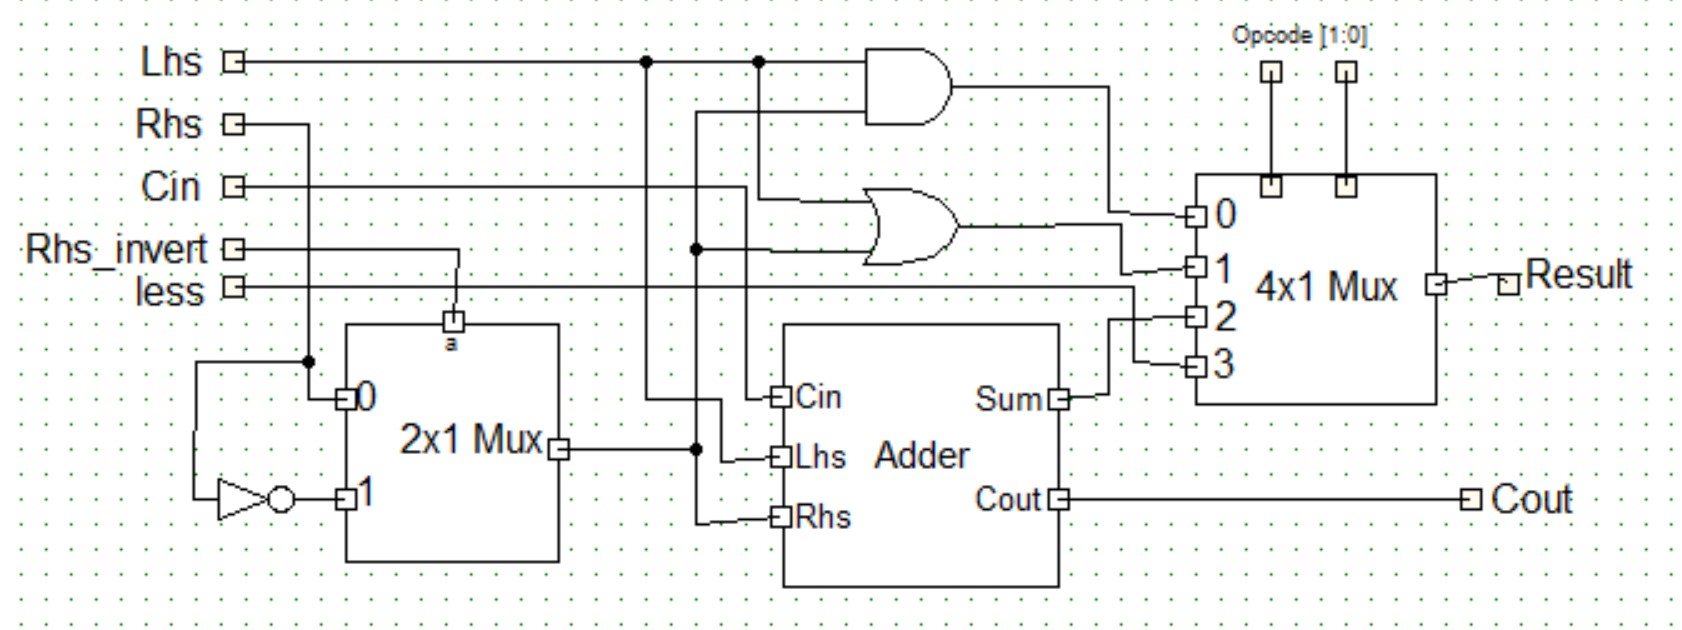
\includegraphics[scale=0.5]{../images/OneBitALU.jpg}\\
        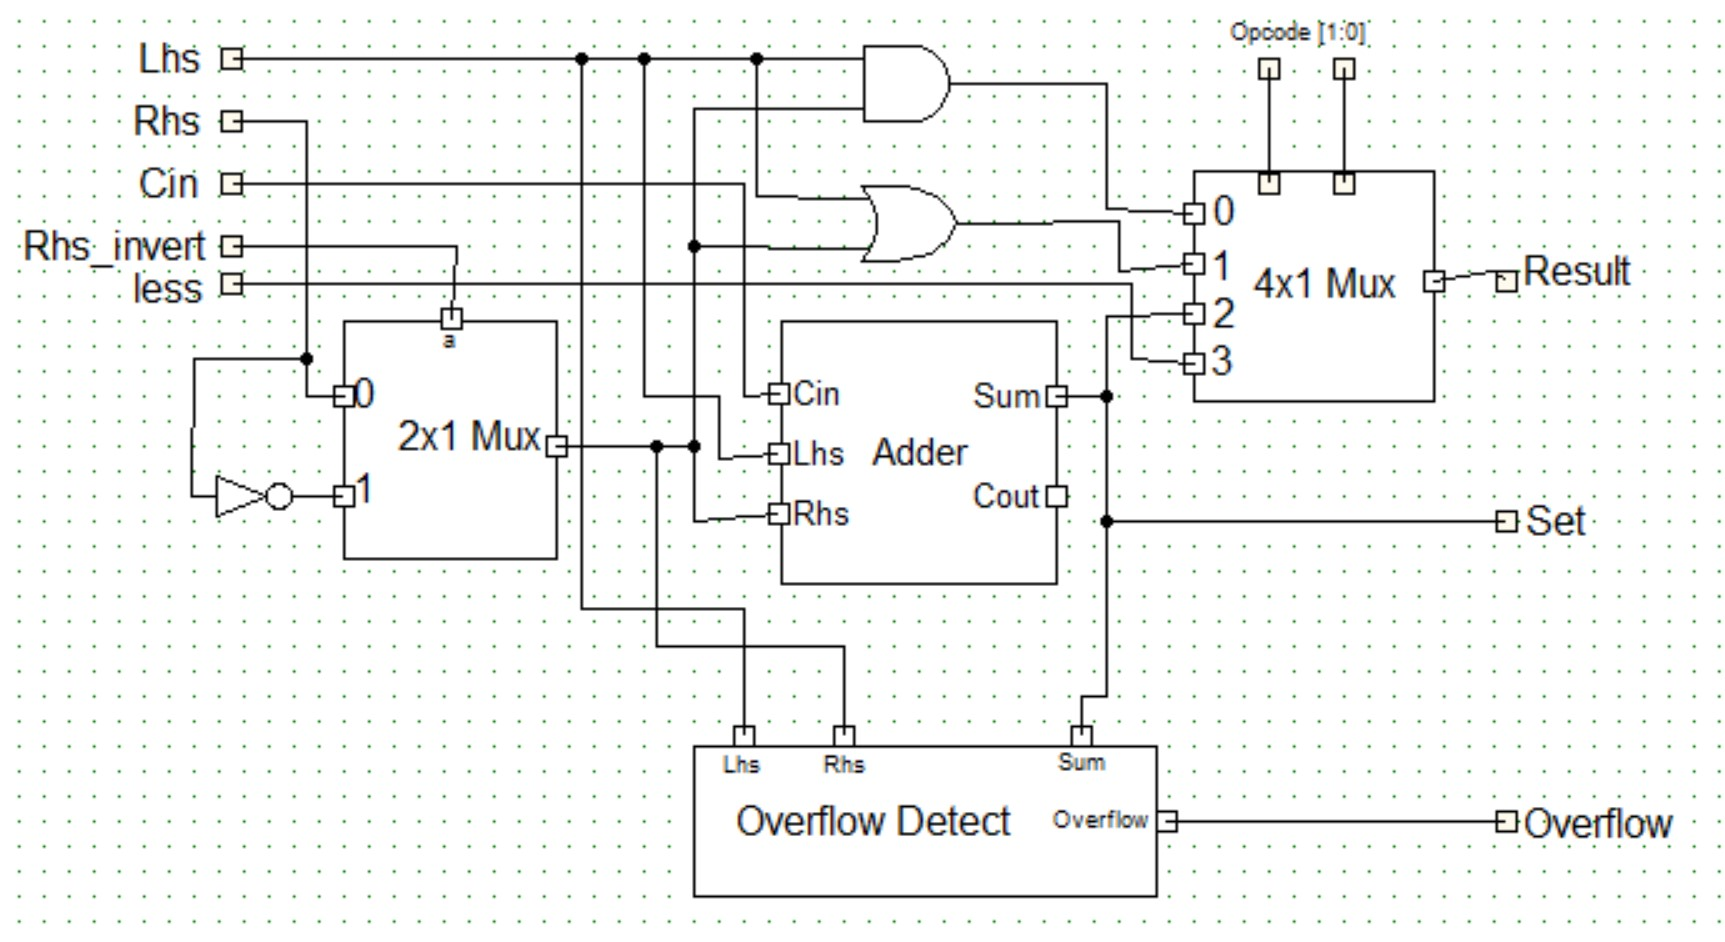
\includegraphics[scale=0.5]{../images/OneBitALU_Set.jpg}
      \end{center}
    \end{problem}
      
  \end{problem}
\end{document}